\documentclass{beamer}

\mode<presentation>
{
  \usetheme{Warsaw}
  \useoutertheme{infolines}
  \usecolortheme[RGB={125,173,51}]{structure}
  %\usetheme[height=7mm]{Rochester}
  % or ...

  \setbeamercovered{transparent}
  % or whatever (possibly just delete it)
}

\usepackage{multicol}
\usepackage{verbatim} 
\usepackage{listings}
\usepackage{tikz}
\usetikzlibrary{arrows}
\usetikzlibrary{shapes}
\tikzstyle{block}=[draw opacity=0.7,line width=1.4cm]

\lstloadlanguages{C++}
\lstnewenvironment{code}
	{%\lstset{	numbers=none, frame=lines, basicstyle=\small\ttfamily, }%
	 \csname lst@SetFirstLabel\endcsname}
	{\csname lst@SaveFirstLabel\endcsname}
\lstset{% general command to set parameter(s)
	language=C++, basicstyle=\footnotesize\ttfamily, keywordstyle=\slshape,
	emph=[1]{tipo,usa}, emphstyle={[1]\sffamily\bfseries},
	morekeywords={tint,forn,forsn},
	basewidth={0.47em,0.40em},
	columns=fixed, fontadjust, resetmargins, xrightmargin=5pt, xleftmargin=15pt,
	flexiblecolumns=false, tabsize=2, breaklines,	breakatwhitespace=false, extendedchars=true,
	numbers=left, numberstyle=\tiny, stepnumber=1, numbersep=9pt,
	frame=l, framesep=3pt,
}

\usepackage[spanish]{babel}
% or whatever

\usepackage[latin1]{inputenc}
% or whatever

\usepackage{times}
\usepackage[T1]{fontenc}
% Or whatever. Note that the encoding and the font should match. If T1
% does not look nice, try deleting the line with the fontenc.


\title{TCO18 Argentina}  % (optional, use only with long paper titles)


\author[Agust�n Guti�rrez] % (optional, use only with lots of authors)
{~Agust�n Santiago Guti�rrez}
% - Give the names in the same order as the appear in the paper.
% - Use the \inst{?} command only if the authors have different
%   affiliation.
\institute[UBA] % (optional, but mostly needed)
{
  %\inst{1}
  Facultad de Ciencias Exactas y Naturales\\
  Universidad de Buenos Aires
}
\date % (optional, should be abbreviation of conference name)
{Agosto 2018}

% Ac� se puede insertar el logo de la UBA
% \pgfdeclareimage[height=0.5cm]{university-logo}{university-logo-filename}
% \logo{\pgfuseimage{university-logo}}



% Delete this, if you do not want the table of contents to pop up at
% the beginning of each subsection:
\AtBeginSubsection[]
{
  \begin{frame}{Contenidos}
  \footnotesize
  \begin{multicols}{2} 
    \tableofcontents[currentsection, currentsubsection]
  \end{multicols}
  \end{frame}
}

\DeclareMathOperator*{\mimin}{min}
\DeclareMathOperator*{\mimax}{max}

% If you wish to uncover everything in a step-wise fashion, uncomment
% the following command: 

%\beamerdefaultoverlayspecification{<+->}


\begin{document}
\pgfdeclarelayer{background}
\pgfsetlayers{background,main}
\begin{frame}
  \titlepage
\end{frame}


\begin{frame}{Estad�sticas}
  \begin{itemize}
     \item 77 participantes registrados
     \item $X$ correctos de $X$ env�os en el problema de 300 puntos
     \item $Y$ correctos de $Y$ env�os en el problema 500 puntos
     \item $Z$ correctos de $Z$ env�os en el problema 1000 puntos
  \end{itemize}
\end{frame}

\begin{frame}{Zeroes of Blight and Tragic}
	Referencia directa a ``Heroes of Might and Magic''
    
    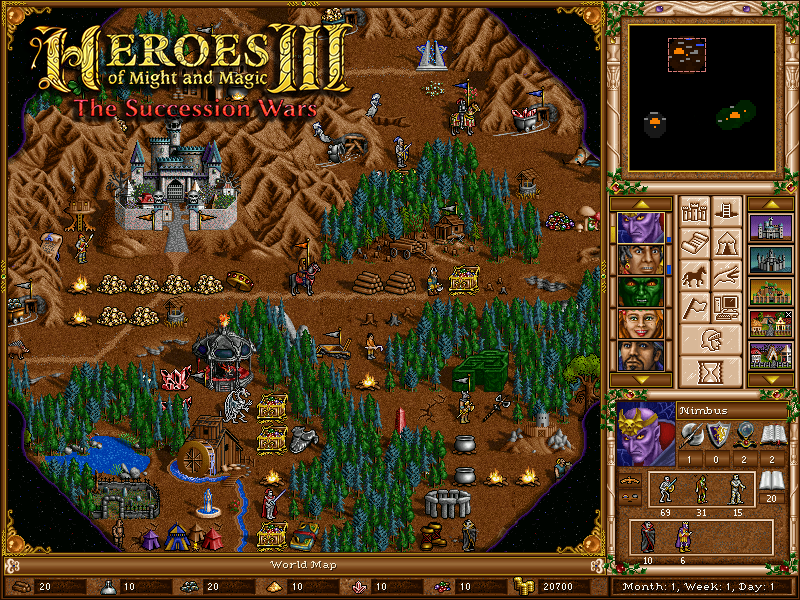
\includegraphics[scale=0.35]{heroes.png}
\end{frame}

\begin{frame}{Zeroes of Blight and Tragic}
	Ejemplos de tama�os:
    
    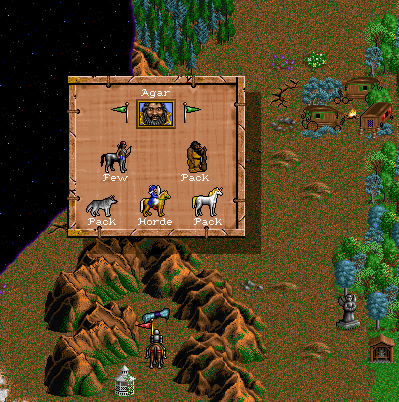
\includegraphics[scale=0.4]{heroes-tam.png}
\end{frame}


\begin{frame}{Idea: suma de intervalos}
    \begin{itemize}
	\item Cada especificador de tama�o indica un \textbf{intervalo}
	\item Si $x \in I_1$, $y \in I_2$, entonces los posibles valores de $x+y$ forman otro intervalo $I_3$.
	\item Se puede calcular $I_3$ sumando los valores extremos de $I_1$ y $I_2$.
    \end{itemize}

\end{frame}


\begin{frame}{Implementando}

    \begin{itemize}
	
    \item Posible implementaci�n: Considerar la suma de los m�nimos, y la suma de los m�ximos.
    \item Iterar el rango de valores de menor a mayor, y para cada uno, obtener el correspondiente String.
    \item Hacer \texttt{v.resize(unique(v.begin(), v.end()) - v.begin());} del arreglo obtenido.
    \item Truquito de implementaci�n: En lugar de hacer muchos ifs a mano, directamnete copy pastear el texto del enunciado con la tabla, y parsearlo.
        \begin{itemize}
            \item Seg�n la pr�ctica y el lenguaje, se hace m�s r�pido que armar muchos ifs a mano
            \item Menos propenso a que nos quede un bug (como ingresar mal un n�mero)
        \end{itemize}
    \end{itemize}
\end{frame}

\begin{frame}{Knishop}
    \begin{itemize}
    \item Observaci�n clave 1: Usar los colores del tablero de ajedrez.
       \begin{itemize}
           \item El caballo \textbf{s� o s�} cambia de color al mover.
           \item El alfil \textbf{jam�s} cambia de color.
       \end{itemize}
    \item Observaci�n clave 2: El alfil puede llegar a cualquier lugar del mismo color en solo 2 movimientos. 
    \end{itemize}
\end{frame}

\begin{frame}
    \begin{itemize}
    \item La respuesta es a lo sumo 3:
        \begin{itemize}
            \item Si inicio $=$ fin, entonces es 0.
            \item Si estamos a un salto de caballo, o bien $|\Delta_x| = |\Delta_y|$, entonces es 1.
            \item Sino, hay que ver si se puede con 2.
                \begin{itemize}
                    \item Si la casilla inicial y final tienen el mismo color, se puede en 2.
                    \item Sino, hay que hacer un salto de caballo, y luego de eso tiene que ser $|\Delta_x| = |\Delta_y|$
                    \item Notar que caballo $+$ alfil $=$ alfil + caballo, y hacer dos movimientos de caballo no sirve (no cambia color). 
                \end{itemize}
            \item Si no se pudo en 2, la respuesta es 3.
        \end{itemize}
	\end{itemize}
\end{frame}

\begin{frame}{ProbabilisticAlice}
    \begin{itemize}
        \item A veces las cosas salen bien, y ganamos sin que nos teletransporten al comienzo.
        \item A veces salen mal, y es un \textbf{fallo}.
        \item Clave: la situaci�n al comenzar otra vez es \textbf{siempre la misma. No hay memoria.}
        \item Es decir, siempre tenemos \textbf{la misma probabilida de �xito}.
        \item La cantidad de intentos hasta tener �xito tiene distribuci�n geom�trica.
        \item $E = 1/p$
    \end{itemize}
\end{frame}

\begin{frame}{C�lculo de $p$}
    \begin{itemize}
        \item Se puede calcular la probabilidad de �xito usando programaci�n din�mica.
    \end{itemize}
\end{frame}

\end{document}
